\chapter{Statistical Inference} 
\chaptermark{Inference}
\label{sec:inference}

The idea of extrapolating knowledge from a \emph{sample} to a population is known as \emph{statistical inference}.
It encompasses the ideas of \emph{parameter estimation}, \emph{confidence intervals}, and \emph{hypothesis testing}.
We will assume the reader is familiar with these, but recall some required terminology.
The QC and SPC terminology are not always consistent with statisticians' terminology. When new names are given to old ideas, we will emphasize this in the text.

\begin{description}
\item [Null/Alternative Hypothesis] Some statement about the world we wish to test with data. The frequentist argument follows a Popperian philosophy\footnote{Following Karl Popper's philosophy of science, we can never know that something is true, we can only know when it is not true. Popper philosophy was motivated by the fact that no one suspected Isaac Newton's mechanics to be wrong, until relativity theory was proposed by Einstein.}: to show the alternative hypothesis is true, we will show that the null hypothesis is not true. 
In the context of quality control, the null hypothesis will be the process is \emph{in statistical control}, while the alternative will be that it is \emph{out of control}.\marginnote{In Control}
Other terms for the alternative hypothesis are the \emph{research hypothesis}, or simply the \emph{signal}.
\item [Statistical Test] The procedure of inferring from data on the truthfulness of the alternative hypothesis.
\item [Assumptions] As the name suggests, these are assumptions. We stress that unlike hypothesis, assumptions are not being tested in a statistical test. 
\item [Test Statistic] The function of the data to be computed for the purpose of inference. As such, it is a random variable. 
May also be though of as a \emph{signal detector}.
\item [Null/Alternative Distribution] The distribution of the test statistic under the null/alternative hypothesis.
\item [Type I/II error] See Figure~\ref{fig:confusion_table}.
\item [False/True Positive/Negative] See Figure~\ref{fig:confusion_table}.
\item [Rejection Region] The collection of event that will lead us to reject the null hypothesis, and believe in the alternative hypothesis.
\item [p-value] A.k.a. \emph{observed significance}. The null probability of the observed (or ``more extreme'') event.
\item [Significance Level] A.k.a. $\alpha$. The probability of a false positive.
\item [Power] The probability of a true positive.
\item [i.i.d.] ``Independent and identically distributed'' (i.i.d.) is an assumption made on the sampling distribution, meaning that samples are statistically independent, and all originating from the same distribution.

\end{description}

\begin{figure}
\centering
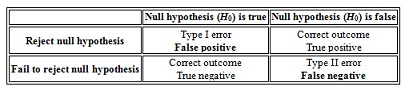
\includegraphics[width=0.8\linewidth]{art/Beware-of-False-Positives-Chart-1}
\caption[Confusion Table]{Type I/II error confusion table. \newline \url{https://infocus.emc.com/william_schmarzo/beware-of-false-positives/}}
\label{fig:confusion_table}
\end{figure}


\begin{extra}[ROC termininology]
%TODO: ROC terminology

The engineering, statistical, and information retrieval literature, define error and precision criteria\footnote{\url{https://en.wikipedia.org/wiki/Receiver_operating_characteristic}}:
\begin{description}
	\item[True Positive Rate] ...
	\item[Sensitivity] ...
	\item[Recall] ...
	\item[False Positive Rate] ...
	\item[Fallout] ...
	\item[Specificity]
	\item[Miss Rate]
	\item[Prevalence]
	\item[True Negative Rate]
	\item[Accuracy]
	\item[Positive Predictive Value]
	\item[Precision] 
	\item[False Omission rate]
	\item[False Discovery Rate]
	\item[Negative Predictive Value]
	\item[Positive Likelihood Ratio]
	\item[Negative Likelihood ratio]
	\item[Disgnostic odds ratio]
\end{description}
\end{extra}


The following sections of this chapter present particular statistical inference methods we will be using in the following chapters.


\begin{think}
Can you design a test with type I error larger its power?
Would you ever want such a test?
Think about it using the analogy to statistical tests and criminal courts. 
\end{think}


